\let\negmedspace\undefined
\let\negthickspace\undefined
\documentclass[journal]{IEEEtran}
\usepackage[a5paper, margin=10mm, onecolumn]{geometry}
\usepackage{tfrupee} 

\setlength{\headheight}{1cm} 
\setlength{\headsep}{0mm}  
\usepackage{gvv-book}
\usepackage{gvv}
\usepackage{cite}
\usepackage{amsmath,amssymb,amsfonts,amsthm}
\usepackage{algorithmic}
\usepackage{graphicx}
\usepackage{textcomp}
\usepackage{xcolor}
\usepackage{txfonts}
\usepackage{listings}
\usepackage{enumitem}
\usepackage{mathtools}
\usepackage{gensymb}
\usepackage{comment}
\usepackage[breaklinks=true]{hyperref}
\usepackage{tkz-euclide} 
\usepackage{listings}
% \usepackage{gvv}                                        
\def\inputGnumericTable{}                                 
\usepackage[latin1]{inputenc}                                
\usepackage{color}                                            
\usepackage{array}                                            
\usepackage{longtable}                                       
\usepackage{calc}                                             
\usepackage{multirow}                                         
\usepackage{hhline}                                           
\usepackage{ifthen}                                           
\usepackage{lscape}
\usepackage{tikz}
\usetikzlibrary{patterns}
\begin{document}

\bibliographystyle{IEEEtran}
\vspace{3cm}


\title{GATE 2009 ME }
\author{ee25btech11029- Jnanesh Sathisha Karmar}
\maketitle
% \maketitle
% \newpage
% \bigskip
{\let\newpage\relax\maketitle}

\renewcommand{\thefigure}{\theenumi}
\renewcommand{\thetable}{\theenumi}
\setlength{\intextsep}{10pt} % Space between text and floats
\begin{enumerate}[leftmargin=0pt]


% Q1
\item The partial differential equation $\dfrac{\partial^2 u}{\partial x^2} = \dfrac{\partial u}{\partial t} + u\,\dfrac{\partial u}{\partial x}$ is a
\begin{enumerate}
\begin{multicols}{2}
\item linear equation of order $2$
\item non-linear equation of order $1$
\item linear equation of order $1$
\item non-linear equation of order $2$
\end{multicols}
\end{enumerate}

\hfill{\brak{\text{GATE ME 2013}}}

% Q2
\item The eigenvalues of a symmetric matrix are all
\begin{enumerate}
\item complex with non-zero positive imaginary part
\item complex with non-zero negative imaginary part
\item real
\item pure imaginary

\end{enumerate}

\hfill{\brak{\text{GATE ME 2013}}}

% Q3
\item Match the \text{CORRECT} pairs.

\begin{table}[h]
    \centering
    \begin{tabular}[12pt]{ |c| c| c| c| }
\hline
$\beta$ & Airplane A & Airplane B & Airplane C \\
\hline
$\beta = -5\,\mathrm{deg}$ & $-0.030$ & $-0.025$ & $0.040$\\
\hline
$\beta = 0\,\mathrm{deg}$ & $0$ & $0$ & $0$ \\
\hline
$\beta = 5\,\mathrm{deg}$ & $0.030$ & $0.025$ & $-0.040$\\
\hline
\end{tabular}

\end{table}
\begin{enumerate}
\begin{multicols}{4}
\item P-$2$, Q-$1$, R-$3$
\item P-$3$, Q-$2$, R-$1$
\item P-$1$, Q-$2$, R-$3$
\item P-$3$, Q-$1$, R-$2$
\end{multicols}
\end{enumerate}

\hfill{\brak{\text{GATE ME 2013}}}

% Q4
\item A rod of length $L$ having uniform cross-sectional area $A$ is subjected to a tensile force $P$ as shown in the figure below. If the Young's modulus of the material varies linearly from $E_1$ to $E_2$ along the length of the rod, the normal stress developed at the section-SS is
\begin{figure}[h]
\centering
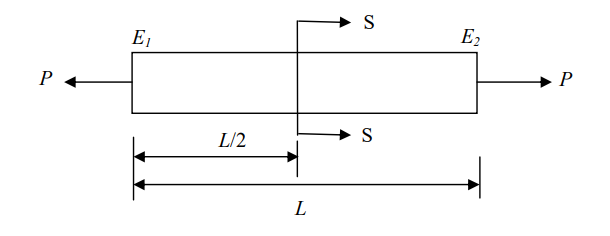
\includegraphics[width=0.5\columnwidth]{Figs/image (14).png}
\caption*{}
\label{fig:5}
\end{figure}

\begin{enumerate}
\begin{multicols}{4}
\item $\dfrac{P}{A}$
\item $\dfrac{\brak{E_2 - E_1}P}{\brak{E_1 + E_2}A}$
\item $\dfrac{E_1}{2E_2}\,\dfrac{P}{A}$
\item $\dfrac{E_2}{2E_1}\,\dfrac{P}{A}$
\end{multicols}
\end{enumerate}

\hfill{\brak{\text{GATE ME 2013}}}
% Q5
\item Two threaded bolts A and B of same material and length are subjected to identical tensile load. If the elastic strain energy stored in bolt A is $4$ times that of bolt B and the mean diameter of bolt A is $12\,\text{mm}$, the mean diameter of bolt B in mm is
\begin{enumerate}
\begin{multicols}{4}
\item $16$
\item $24$
\item $36$
\item $48$
\end{multicols}
\end{enumerate}

\hfill{\brak{\text{GATE ME 2013}}}

% Q6
\item A link OB is rotating with a constant angular velocity of $2\,\text{rad/s}$ in counter clockwise direction and a block is sliding radially outward on it with a uniform velocity of $0.75\,\text{m/s}$ with respect to the rod, as shown in the figure below. If $OA = 1\,\text{m}$, the magnitude of the absolute acceleration of the block at location A in $\text{m/s}^2$ is
\begin{figure}[h]
    \centering
    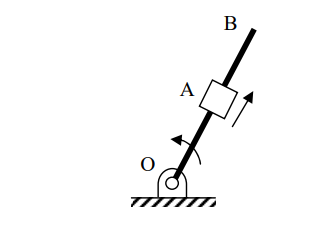
\includegraphics[width=0.5\columnwidth]{Figs/image (15).png}
    \caption*{}
    \label{fig:q6}
\end{figure}
\begin{enumerate}
\begin{multicols}{4}
\item $3$
\item $4$
\item $5$
\item $6$
\end{multicols}
\end{enumerate}

\hfill{\brak{\text{GATE ME 2013}}}

% Q7
\item For steady, fully developed flow inside a straight pipe of diameter $D$, neglecting gravity effects, the pressure drop $\Delta p$ over a length $L$ and the wall shear stress $\tau_w$ are related by
\begin{enumerate}
\begin{multicols}{4}
\item $\tau_w = \dfrac{\Delta p\, D}{4L}$
\item $\tau_w = \dfrac{\Delta p\, D^2}{4L}$
\item $\tau_w = \dfrac{\Delta p\, D}{2L}$
\item $\tau_w = \dfrac{\Delta p\, L}{4D}$
\end{multicols}
\end{enumerate}

\hfill{\brak{\text{GATE ME 2013}}}

% Q8
\item The pressure, dry bulb temperature and relative humidity of air in a room are $1\,\text{bar}$, $30\degree\,\text{C}$ and $70\%$, respectively. If the saturated steam pressure at $30\degree\,\text{C}$ is $4.25\,\text{kPa}$, the specific humidity of the room air in $\text{kg water vapour}/\text{kg dry air}$ is
\begin{enumerate}
\begin{multicols}{4}
\item $0.0083$
\item $0.0101$
\item $0.0191$
\item $0.0232$
\end{multicols}
\end{enumerate}

\hfill{\brak{\text{GATE ME 2013}}}

% Q9
\item Consider one-dimensional steady state heat conduction, without heat generation, in a plane wall; with boundary conditions as shown in the figure below. The conductivity of the wall is given by $k = k_0 + bT$; where $k_0$ and $b$ are positive constants, and $T$ is temperature. As $x$ increases, the temperature gradient $\brak{\dfrac{dT}{dx}}$ will
\begin{figure}[h]
\centering
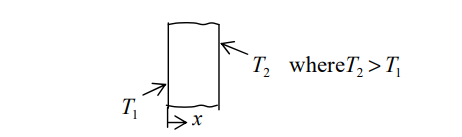
\includegraphics[width=0.5\columnwidth]{Figs/image (19).png}
\caption*{}
\label{fig:9}
\end{figure}
\begin{enumerate}
\begin{multicols}{4}
\item remain constant
\item be zero
\item increase
\item decrease
\end{multicols}
\end{enumerate}

\hfill{\brak{\text{GATE ME 2013}}}

% Q10
\item In a rolling process, the state of stress of the material undergoing deformation is
\begin{enumerate}
\begin{multicols}{2}
\item pure compression
\item pure shear
\item compression and shear
\item tension and shear
\end{multicols}
\end{enumerate}

\hfill{\brak{\text{GATE ME 2013}}}

% Q11
\item Match the \text{CORRECT} pairs.

\begin{table}[h]
    \centering
    \begin{table}[h!]
\small
\setlength{\tabcolsep}{4pt}
\renewcommand{\arraystretch}{0.9}
\centering
\begin{tabular}{|c|c|c|p{1.8cm}|p{2.5cm}|c|}
\hline
Q. No & Type & Section & Key & Marks \\
\hline
1  & MCQ & GA & C         & 1 \\
\hline
2  & MCQ & GA & A         & 1 \\
\hline
3  & MCQ & GA & A         & 1 \\
\hline
4  & MCQ & GA & A         & 1 \\
\hline
5  & MCQ & GA & D         & 1 \\
\hline
6  & MCQ & GA & D         & \textbf{2} \\
\hline
7  & MCQ & GA & B         & 2 \\
\hline
8  & MCQ & GA & C         & 2 \\
\hline
9  & MCQ & GA & B         & 2 \\
\hline
10 & MCQ & GA & C         & 2 \\
\hline
11 & MCQ & EY & D         & 1 \\
\hline
12 & MCQ & EY & D         & 1 \\
\hline
13 & MCQ & EY & A; D      & 1 \\
\hline
14 & MCQ & EY & B         & 1 \\
\hline
15 & NAT & EY & 7.99 : 8.10 & 1 \\
\hline
16 & MCQ & EY & B         & 1 \\
\hline
17 & MCQ & EY & C         & 1 \\
\hline
18 & MCQ & EY & D         & 1 \\
\hline
19 & NAT & EY & 9.9 : 10.1  & 1 \\
\hline
20 & MCQ & EY & C         & 1 \\
\hline
21 & MCQ & EY & B         & 1 \\
\hline
22 & MCQ & EY & A         & 1 \\
\hline
23 & MCQ & EY & D         & 1 \\
\hline
24 & MCQ & EY & B         & 1 \\
\hline
25 & MCQ & EY & A         & 1 \\
\hline
26 & MCQ & EY & C         & 2 \\
\hline
27 & MCQ & EY & D         & 2 \\
\hline
28 & MCQ & EY & C         & 2 \\
\hline
29 & MCQ & EY & D         & 2 \\
\hline
30 & MCQ & EY & B         & 2 \\
\hline
31 & MCQ & EY & A         & 2 \\
\hline
32 & MCQ & EY & C         & 2 \\
\hline
33 & MCQ & EY & A         & 2 \\
\hline
34 & MCQ & EY & B         & 2 \\
\hline
35 & MCQ & EY & A         & 2 \\
\hline
36 & MCQ & EY & A         & 2 \\
\hline
37 & MCQ & EY & C         & 2 \\
\hline
38 & MCQ & EY & A         & 2 \\
\hline
39 & NAT & EY & 0.17 : 0.19 & 2 \\
\hline
40 & MCQ & EY & A         & 2 \\
\hline
41 & MCQ & EY & B         & 2 \\
\hline
42 & MCQ & EY & B         & 2 \\
\hline
43 & MCQ & EY & A         & 2 \\
\hline
44 & MCQ & EY & D         & 2 \\
\hline
45 & MCQ & EY & B         & 2 \\
\hline
46 & MCQ & EY & A         & 2 \\
\hline
47 & NAT & EY & 0.175 : 0.20 & 2 \\
\hline
48 & MCQ & EY & A         & 2 \\
\hline
49 & NAT & EY & 0.49 : 0.51  & 2 \\
\hline
50 & MCQ & EY & B         & 2 \\
\hline
51 & MCQ & EY & A         & 2 \\
\hline
52 & MCQ & EY & C         & 2 \\
\hline
53 & NAT & EY & 1660 : 1700 & 2 \\
\hline
54 & NAT & EY & 0.45 : 0.55 & 2 \\
\hline
55 & MCQ & EY & A         & 2 \\
\hline
\end{tabular}
\caption{GATE 2016 EY Answer Key Summary}
\end{table}
\end{table}
\begin{enumerate}
\begin{multicols}{2}
\item P-$4$, Q-$3$, R-$1$, S-$2$
\item P-$4$, Q-$2$, R-$3$, S-$1$
\item P-$2$, Q-$3$, R-$4$, S-$1$
\item P-$2$, Q-$4$, R-$1$, S-$3$
\end{multicols}
\end{enumerate}

\hfill{\brak{\text{GATE ME 2013}}}

\item A metric thread of pitch $2$ mm and thread angle $60\degree$ is inspected for its pitch diameter using 3-wire method. The diameter of the best size wire in mm is 
\begin{enumerate}
\begin{multicols}{4}
\item $0.866$
\item $1.000$
\item $1.154$
\item $2.000$
\end{multicols}
\end{enumerate}
\hfill{\brak{\text{GATE ME 2013}}}

\item Customers arrive at a ticket counter at a rate of $50$ per hr and tickets are issued in the order of their arrival. The average time taken for issuing a ticket is $1$ min. Assuming that customer arrivals form a Poisson process and service times are exponentially distributed, the average waiting time in queue in min is 
\begin{enumerate}
\begin{multicols}{4}
\item $3$
\item $4$
\item $5$
\item $6$
\end{multicols}
\end{enumerate}
\hfill{\brak{\text{GATE ME 2013}}}

\item In simple exponential smoothing forecasting, to give higher weightage to recent demand information, the smoothing constant must be close to 
\begin{enumerate}
\begin{multicols}{4}
\item $-1$
\item $0$
\item $0.5$
\item $1.0$
\end{multicols}
\end{enumerate}
\hfill{\brak{\text{GATE ME 2013}}}

\item A steel bar 200 mm in diameter is turned at a feed of $0.25$ mm/rev with a depth of cut of $4$ mm. The rotational speed of the workpiece is $160$ rpm. The material removal rate in mm$^3$/s is 
\begin{enumerate}
\begin{multicols}{4}
\item $160$
\item $167.6$
\item $1600$
\item $1675.5$
\end{multicols}
\end{enumerate}
\hfill{\brak{\text{GATE ME 2013}}}

\item A cube shaped casting solidifies in $5$ min. The solidification time in min for a cube of the same material, which is $8$ times heavier than the original casting, will be 
\begin{enumerate}
\begin{multicols}{4}
\item $10$
\item $20$
\item $24$
\item $40$
\end{multicols}
\end{enumerate}
\hfill{\brak{\text{GATE ME 2013}}}

\item For a ductile material, toughness is a measure of 
\begin{enumerate}
\begin{multicols}{2}
\item resistance to scratching
\item ability to absorb energy up to fracture
\item ability to absorb energy till elastic limit
\item resistance to indentation
\end{multicols}
\end{enumerate}
\hfill{\brak{\text{GATE ME 2013}}}

\item In order to have maximum power from a Pelton turbine, the bucket speed must be 
\begin{enumerate}
\begin{multicols}{2}
\item equal to the jet speed.
\item equal to half of the jet speed.
\item equal to twice the jet speed.
\item independent of the jet speed.
\end{multicols}
\end{enumerate}
\hfill{\brak{\text{GATE ME 2013}}}

\item Consider one-dimensional steady state heat conduction along x-axis $0 \leq x \leq L$, through a plane wall with the boundary surfaces $x=0$ and $x=L$ maintained at temperatures $0\degree$C and $100\degree$C. Heat is generated uniformly throughout the wall. Choose the CORRECT statement.
\begin{enumerate}
\begin{multicols}{2}
\item The direction of heat transfer will be from the surface at $100\degree$C to the surface at $0\degree$C.
\item The maximum temperature inside the wall must be greater than $100\degree$C.
\item The temperature distribution is linear within the wall.
\item The temperature distribution is symmetric about the mid-plane of the wall.
\end{multicols}
\end{enumerate}
\hfill{\brak{\text{GATE ME 2013}}}

\item A cylinder contains $5$ m$^3$ of an ideal gas at a pressure of $1$ bar. This gas is compressed in a reversible isothermal process till its pressure increases to $5$ bar. The work in kJ required for this process is
\begin{enumerate}
\begin{multicols}{4}
\item $804.7$
\item $953.2$
\item $981.7$
\item $1012.2$
\end{multicols}
\end{enumerate}
\hfill{\brak{\text{GATE ME 2013}}}

\item A long thin walled cylindrical shell, closed at both the ends, is subjected to an internal pressure. The ratio of the hoop stress (circumferential stress) to longitudinal stress developed in the shell is
\begin{enumerate}
\begin{multicols}{4}
\item $0.5$
\item $1.0$
\item $2.0$
\item $4.0$
\end{multicols}
\end{enumerate}
\hfill{\brak{\text{GATE ME 2013}}}




\item If two nodes are observed at a frequency of $1800$ rpm during whirling of a simply supported long slender rotating shaft, the first critical speed of the shaft in rpm is
\begin{enumerate}
\begin{multicols}{4}
\item $200$
\item $450$
\item $600$
\item $900$
\end{multicols}
\end{enumerate}
\hfill{\brak{\text{GATE ME 2013}}}

\item A planar closed kinematic chain is formed with rigid links $PQ = 2.0$ m, $QR = 3.0$ m, $RS = 2.5$ m and $SP = 2.7$ m with all revolute joints. The link to be fixed to obtain a double rocker \brak{\text{rocker-rocker}} mechanism is
\begin{enumerate}
\begin{multicols}{4}
\item $PQ$
\item $QR$
\item $RS$
\item $SP$
\end{multicols}
\end{enumerate}
\hfill{\brak{\text{GATE ME 2013}}}

\item Let $X$ be a normal random variable with mean $1$ and variance $4$. The probability $P\{X < 0\}$ is
\begin{enumerate}
\begin{multicols}{2}
\item $0.5$
\item greater than zero and less than $0.5$
\item greater than $0.5$ and less than $1.0$
\item $1.0$
\end{multicols}
\end{enumerate}
\hfill{\brak{\text{GATE ME 2013}}}

\item Choose the CORRECT set of functions, which are linearly dependent.
\begin{enumerate}
\begin{multicols}{2}
\item $x \sin x$, $2 \sin x$ and $2 \cos x$
\item $\cos x$, $x \sin x$ and $x \tan x$
\item $\cos 2x$, $2 \sin x$ and $2 \cos x$
\item $\cos 2x$, $x \sin x$ and $x \cos x$
\end{multicols}
\end{enumerate}
\hfill{\brak{\text{GATE ME 2013}}}

\item The following surface integral is to be evaluated over a sphere for the given steady velocity vector field $\mathbf{F} = x \mathbf{i} + y \mathbf{j} + z \mathbf{k}$ defined with respect to a Cartesian coordinate system having $\mathbf{i}$, $\mathbf{j}$ and $\mathbf{k}$ as unit base vectors.
\begin{align*}
\frac14 \iint_S (\mathbf{F} \cdot \mathbf{n}) \, dA
\end{align*}
where $S$ is the sphere, $x^2 + y^2 + z^2 = 1$ and $\mathbf{n}$ is the outward unit normal vector to the sphere. The value of the surface integral is
\begin{enumerate}
\begin{multicols}{4}
\item $\pi$
\item $2\pi$
\item $\frac{3\pi}{4}$
\item $4\pi$
\end{multicols}
\end{enumerate}
\hfill{\brak{\text{GATE ME 2013}}}

\item The function $f(t)$ satisfies the differential equation
\begin{align*}
\frac{d^2 f}{dt^2} + f = 0
\end{align*}
and the auxiliary conditions $f(0) = 0,\ \frac{df}{dt}(0) = 4$. The Laplace transform of $f(t)$ is given by
\begin{enumerate}
\begin{multicols}{4}
\item $\frac{1}{s^2 + 1}$
\item $\frac{4}{s^2 + 1}$
\item $\frac{1}{s^2 + 4}$
\item $\frac{4}{s^2 + 4}$
\end{multicols}
\end{enumerate}
\hfill{\brak{\text{GATE ME 2013}}}

\item Specific enthalpy and velocity of steam at inlet and exit of a steam turbine, running under steady state, are as given below:

\begin{table}[h!]
\centering
\caption*{}
\label{tab:q28}
\begin{tabular}{c c c}
 & \textbf{Specific enthalpy (kJ/kg)} & \textbf{Velocity (m/s)} \\
\textbf{Inlet} & $3250$ & $180$ \\
\textbf{Exit} & $2360$ & $5$ \\
\end{tabular}
\end{table}

The rate of heat loss from the turbine per kg of steam flow rate is $5$ kW. Neglecting changes in potential energy of steam, the power developed in kW by the steam turbine per kg of steam flow rate is
\begin{enumerate}
\begin{multicols}{4}
\item $901.2$
\item $911.2$
\item $17072.5$
\item $17082.5$
\end{multicols}
\end{enumerate}
\hfill{\brak{\text{GATE ME 2013}}}

\item Water is coming out from a tap and falls vertically downwards. At the tap opening, the stream diameter is $20$ mm with uniform velocity of $2$ m/s. Acceleration due to gravity is $9.81$ m/s$^2$. Assuming steady, inviscid flow, constant atmospheric pressure everywhere and neglecting curvature and surface tension effects, the diameter in mm of the stream $0.5$ m below the tap is approximately
\begin{enumerate}
\begin{multicols}{4}
\item $10$
\item $15$
\item $20$
\item $25$
\end{multicols}
\end{enumerate}
\hfill{\brak{\text{GATE ME 2013}}}

\item A steel ball of diameter $60$ mm is initially in thermal equilibrium at $1030\degree$C in a furnace. It is suddenly removed from the furnace and cooled in ambient air at $30\degree$C, with convective heat transfer coefficient $h = 20$ W/m$^2$K. The thermo-physical properties of steel are: density $\rho = 7800$ kg/m$^3$, conductivity $k = 40$ W/mK and specific heat $c = 600$ J/kgK. The time required in seconds to cool the steel ball in air from $1030\degree$C to $430\degree$C is
\begin{enumerate}
\begin{multicols}{4}
\item $519$
\item $931$
\item $1195$
\item $2144$
\end{multicols}
\end{enumerate}
\hfill{\brak{\text{GATE ME 2013}}}

\item A flywheel connected to a punching machine has to supply energy of $400$ Nm while running at a mean angular speed of $20$ rad/s. If the total fluctuation of speed is not to exceed $\pm 2\%$, the mass moment of inertia of the flywheel in kg-m$^2$ is
\begin{enumerate}
\begin{multicols}{4}
\item $25$
\item $50$
\item $100$
\item $125$
\end{multicols}
\end{enumerate}
\hfill{\brak{\text{GATE ME 2013}}}

\item A compound gear train with gears P, Q, R and S has number of teeth $20$, $40$, $15$ and $20$, respectively. Gears Q and R are mounted on the same shaft as shown in the figure below. The diameter of the gear Q is twice that of the gear R. If the module of the gear R is $2$ mm, the center distance in mm between gears P and S is

\begin{figure}[h]
\centering
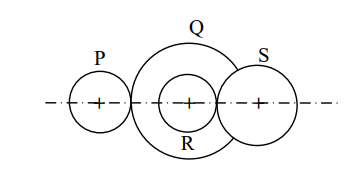
\includegraphics[width=0.5\columnwidth]{Figs/image (18).png}
\caption*{}
\label{fig:32}
\end{figure}
\begin{enumerate}
\begin{multicols}{4}
\item $40$
\item $80$
\item $120$
\item $160$
\end{multicols}
\end{enumerate}
\hfill{\brak{\text{GATE ME 2013}}}


\item A pin jointed uniform rigid rod of weight $W$ and length $l$ is supported horizontally by an external force $F$ as shown in the figure below. The force $F$ is suddenly removed. At the instant of force removal, the magnitude of vertical reaction developed at the support is
\begin{figure}[h]
\centering
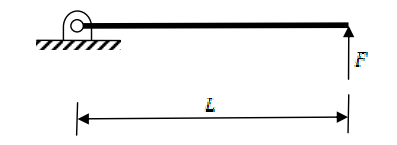
\includegraphics[width=0.5\columnwidth]{Figs/image (20).png}
\caption*{}
\label{fig:33}
\end{figure}
\begin{enumerate}
\begin{multicols}{4}
\item zero
\item $\frac{W}{4}$
\item $\frac{W}{2}$
\item $W$
\end{multicols}
\end{enumerate}

\hfill{\brak{\text{GATE ME 2013}}}

\item Two cutting tools are being compared for a machining operation. The tool life equations are:
\begin{align*}
&\text{Carbide tool:}\quad VT^{1.6} = 3000 \\
&\text{HSS tool:}\quad VT^{0.6} = 200
\end{align*}
where $V$ is the cutting speed in m/min and $T$ is the tool life in min. The carbide tool will provide higher tool life if the cutting speed in m/min exceeds
\begin{enumerate}
\begin{multicols}{4}
\item $15.0$
\item $39.4$
\item $49.3$
\item $60.0$
\end{multicols}
\end{enumerate}
\hfill{\brak{\text{GATE ME 2013}}}

\item In a CAD package, mirror image of a $2D$ point $P\brak{5,10}$ is to be obtained about a line which passes through the origin and makes an angle of $45\degree$ counterclockwise with the $X$-axis. The coordinates of the transformed point will be
\begin{enumerate}
\begin{multicols}{4}
\item $7.5, 5$
\item $10, 5$
\item $7.5, -5$
\item $10, -5$
\end{multicols}
\end{enumerate}
\hfill{\brak{\text{GATE ME 2013}}}

\item A linear programming problem is shown below.
\begin{align*}
&\text{Maximize}\quad 3x + 7y \\
&\text{Subject to}\quad 3x + 7y \leq 10 \\
&4x + 6y \leq 8 \\
&x, y \geq 0
\end{align*}
It has
\begin{enumerate}
\begin{multicols}{4}
\item an unbounded objective function.
\item exactly one optimal solution.
\item exactly two optimal solutions.
\item infinitely many optimal solutions.
\end{multicols}
\end{enumerate}
\hfill{\brak{\text{GATE ME 2013}}}

\item Cylindrical pins of $25^{+0.020}_{+0.010}$ mm diameter are electroplated in a shop. Thickness of the plating is $30 \pm 0.2$ micron. Neglecting gage tolerances, the size of the GO gage in mm to inspect the plated components is
\begin{enumerate}
\begin{multicols}{4}
\item $25.042$
\item $25.052$
\item $25.074$
\item $25.084$
\end{multicols}
\end{enumerate}
\hfill{\brak{\text{GATE ME 2013}}}

\item During the electrochemical machining \brak{\text{ECM}} of iron \brak{\text{atomic weight} = 56,\ \text{valency} = 2} at current of $1000$ A with $90\%$ current efficiency, the material removal rate was observed to be $0.26$ gm/s. If Titanium \brak{\text{atomic weight} = 48,\ \text{valency} = 3} is machined by the ECM process at the current of $2000$ A with $90\%$ current efficiency, the expected material removal rate in gm/s will be
\begin{enumerate}
\begin{multicols}{4}
\item $0.11$
\item $0.23$
\item $0.30$
\item $0.52$
\end{multicols}
\end{enumerate}
\hfill{\brak{\text{GATE ME 2013}}}

\item A single degree of freedom system having mass $1$ kg and stiffness $10$ kN/m initially at rest is subjected to an impulse force of magnitude $5$ kN for $10^{-4}$ seconds. The amplitude in mm of the resulting free vibration is
\begin{enumerate}
\begin{multicols}{4}
\item $0.5$
\item $1.0$
\item $5.0$
\item $10.0$
\end{multicols}
\end{enumerate}
\hfill{\brak{\text{GATE ME 2013}}}

\item A bar is subjected to fluctuating tensile load from $20$ kN to $100$ kN. The material has yield strength of $240$ MPa and endurance limit in reversed bending is $160$ MPa. According to the Soderberg principle, the area of cross-section in mm$^2$ of the bar for a factor of safety of $2$ is
\begin{enumerate}
\begin{multicols}{4}
\item $400$
\item $600$
\item $750$
\item $1000$
\end{multicols}
\end{enumerate}
\hfill{\brak{\text{GATE ME 2013}}}

\item A simply supported beam of length $L$ is subjected to a varying distributed load $\sin\brak{\frac{3 \pi x}{L}}$ N/m, where the distance $x$ is measured from the left support. The magnitude of the vertical reaction force in N at the left support is
\begin{enumerate}
\begin{multicols}{4}
\item zero
\item $\frac{3}{\pi}L$
\item $\frac{\pi}{L}$
\item $\frac{\pi}{2L}$
\end{multicols}
\end{enumerate}
\hfill{\brak{\text{GATE ME 2013}}}

\item Two large diffuse gray parallel plates, separated by a small distance, have surface temperatures of $400$ K and $300$ K. If the emissivities of the surfaces are $0.8$ and the Stefan-Boltzmann constant is $5.67 \times 10^{-8}$ $W/m^2K^4$ , the net radiation heat exchange rate in $kW/m^2$ between the two plates is
\begin{enumerate}
\begin{multicols}{4}
\item $0.66$
\item $0.79$
\item $0.99$
\item $3.96$
\end{multicols}
\end{enumerate}
\hfill{\brak{\text{GATE ME 2013}}}

\item A hinged gate of length $5$ m, inclined at $30\degree$ with the horizontal and with water mass on its left, is shown in the figure below. Density of water is $1000$ kg/m$^3$. The minimum mass of the gate in kg per unit width \brak{\text{perpendicular to the plane of paper}} required to keep it closed is
\begin{figure}[h]
\centering
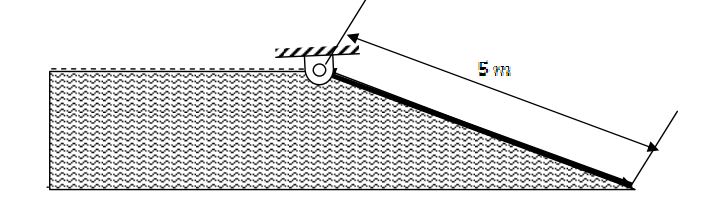
\includegraphics[width=0.5\columnwidth]{Figs/image (17).png}
\caption*{}
\label{fig:43}
\end{figure}
\begin{enumerate}
\begin{multicols}{4}
\item $5000$
\item $6600$
\item $7546$
\item $9623$
\end{multicols}
\end{enumerate}

\hfill{\brak{\text{GATE ME 2013}}}


\item The pressure, temperature and velocity of air flowing in a pipe are $5$ bar, $500$ K and $50$ m/s, respectively. The specific heats of air at constant pressure and at constant volume are $1.005$ kJ/kgK and $0.718$ kJ/kgK, respectively. Neglect potential energy. If the pressure and temperature of the surroundings are $1$ bar and $300$ K, respectively, the available energy in kJ/kg of the air stream is
\begin{enumerate}
\begin{multicols}{4}
\item $170$
\item $187$
\item $191$
\item $213$
\end{multicols}
\end{enumerate}
\hfill{\brak{\text{GATE ME 2013}}}

\item The probability that a student knows the correct answer to a multiple choice question is $\frac{2}{3}$. If the student does not know the answer, then the student guesses the answer. The probability of the guessed answer being correct is $\frac14$. Given that the student has answered the question correctly, the conditional probability that the student knows the correct answer is
\begin{enumerate}
\begin{multicols}{4}
\item $\frac{2}{3}$
\item $\frac{3}{4}$
\item $\frac{5}{6}$
\item $\frac{8}{9}$
\end{multicols}
\end{enumerate}
\hfill{\brak{\text{GATE ME 2013}}}

\item The solution to the differential equation
\begin{align*}
\frac{d^2u}{dx^2} - k\frac{du}{dx} = 0
\end{align*}
where $k$ is a constant, subjected to the boundary conditions $u(0) = 0$ and $u(L) = U$, is
\begin{enumerate}
\begin{multicols}{4}
\item $\frac{U}{L}x$
\item $U\frac{e^{-kL} - e^{-kx}}{e^{-kL} - 1}$
\item $U\frac{e^{kL} - e^{kx}}{e^{kL} - 1}$
\item $U\frac{e^{kL} + e^{kx}}{e^{kL} + 1}$
\end{multicols}
\end{enumerate}
\hfill{\brak{\text{GATE ME 2013}}}

\item The value of the definite integral 
\[
\int_{x=0}^{x=1} \frac{\ln x}{x} \,dx
\]
is
\begin{enumerate}
\begin{multicols}{4}
\item $\frac{3}{4} \ln 9 + 2$
\item $\frac{3}{2} \ln 9 - 4$
\item $\frac{3}{4} \ln 9 + 4$
\item $\frac{3}{2} \ln 9 - 2$
\end{multicols}
\end{enumerate}
\hfill{\brak{\text{GATE ME 2013}}}


\textbf{Common Data for Q48 and Q49:}  
A single riveted lap joint of two similar plates as shown in the figure below has the following geometrical and material details:
width of the plate $w = 200$ mm, thickness of the plate $t=5$ mm, number of rivets $n = 3$, diameter of the rivet $d_r = 10$ mm, diameter of the rivet hole $d_h = 11$ mm, allowable tensile stress of the plate $\sigma_p = 200$ MPa, allowable shear stress of the rivet $\sigma_s = 100$ MPa and allowable bearing stress of the rivet $\sigma_c = 150$ MPa.  
\begin{figure}[h]
\centering
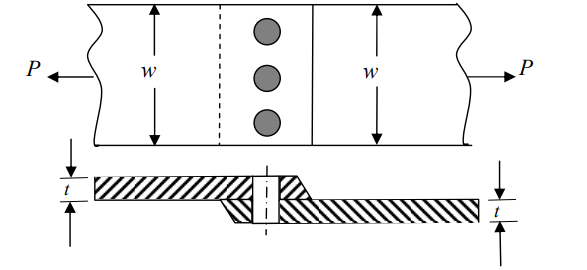
\includegraphics[width=0.45\columnwidth]{Figs/image (21).png}
\caption*{}
\label{fig:48}
\end{figure}

\item 




If the rivets are to be designed to avoid crushing failure, the maximum permissible load $P$ in kN is
\begin{enumerate}
\begin{multicols}{4}
\item $7.50$
\item $15.00$
\item $22.50$
\item $30.00$
\end{multicols}
\end{enumerate}
\hfill{\brak{\text{GATE ME 2013}}}

\item If the plates are to be designed to avoid tearing failure, the maximum permissible load $P$ in kN is
\begin{enumerate}
\begin{multicols}{4}
\item $83$
\item $125$
\item $167$
\item $501$
\end{multicols}
\end{enumerate}
\hfill{\brak{\text{GATE ME 2013}}}

\textbf{Common Data for Q50 and Q51:}  \\
Water ($c_p = 4.18$ kJ/kgK) enters a pipe at a rate of $0.01$ kg/s and a temperature of $20\degree$C. The pipe, of diameter $50$ mm and length $3$ m, is subjected to a wall heat flux $q''$ in W/m$^2$.\\
\item


If $q'' = 2500x$, where $x$ is in m and in the direction of flow ($x=0$ at the inlet), the bulk mean temperature of the water leaving the pipe in $\degree$C is
\begin{enumerate}
\begin{multicols}{4}
\item $42$
\item $62$
\item $74$
\item $104$
\end{multicols}
\end{enumerate}
\hfill{\brak{\text{GATE ME 2013}}}

\item If $q'' = 5000$ and the convection heat transfer coefficient at the pipe outlet is $1000$ W/m$^2$K, the temperature in $\degree$C at the inner surface of the pipe at the outlet is
\begin{enumerate}
\begin{multicols}{4}
\item $71$
\item $76$
\item $79$
\item $81$
\end{multicols}
\end{enumerate}
\hfill{\brak{\text{GATE ME 2013}}}

\textbf{Linked Answer Questions Q52 and Q53:}  \\
In orthogonal turning of a bar of $100 mm$ diameter with a feed of $0.25 mm/rev$ , depth of cut of $4 mm$ and cutting velocity of $90 m/min$ , it is observed that the main \brak{tangential} cutting force is perpendicular to the friction force acting at the chip-tool interface. The main cutting force is $1500 N$.\\
\item
The orthogonal rake angle of the cutting tool in degree is
\begin{enumerate}
\begin{multicols}{4}
\item $0$
\item $3.58$
\item $5$
\item $7.16$
\end{multicols}
\end{enumerate}
\hfill{\brak{\text{GATE ME 2013}}}

\item The normal force acting at the chip-tool interface in N is
\begin{enumerate}
\begin{multicols}{4}
\item $1000$
\item $1500$
\item $2000$
\item $2500$
\end{multicols}
\end{enumerate}
\hfill{\brak{\text{GATE ME 2013}}}

\textbf{Linked Answer Questions Q54 and Q55:}  
\item
In a simple Brayton cycle, the pressure ratio is $8$ and temperatures at the entrance of compressor and turbine are $300$ K and $1400$ K, respectively. Both compressor and gas turbine have isentropic efficiencies of $0.8$. For the gas, assume $c_p = 1$ kJ/kgK and $\gamma = 1.4$.

The power required by the compressor in kW per kg of gas flow rate is
\begin{enumerate}
\begin{multicols}{4}
\item $194.7$
\item $243.4$
\item $304.3$
\item $378.5$
\end{multicols}
\end{enumerate}
\hfill{\brak{\text{GATE ME 2013}}}

\item The thermal efficiency of the cycle in \% is
\begin{enumerate}
\begin{multicols}{4}
\item $24.8$
\item $38.6$
\item $44.8$
\item $53.1$
\end{multicols}
\end{enumerate}
\hfill{\brak{\text{GATE ME 2013}}}

\textbf{General Aptitude (GA) Questions}
\item Universalism is to particularism as diffuseness is to \underline{\hspace{2cm}} 
\begin{enumerate}
\begin{multicols}{4}
\item specificity
\item neutrality
\item generality
\item adaptation
\end{multicols}
\end{enumerate}
\hfill{\brak{\text{GATE ME 2013}}}

\item Were you a bird, you \underline{\hspace{2cm}} in the sky.
\begin{enumerate}
\begin{multicols}{4}
\item would fly
\item shall fly
\item should fly
\item shall have flown
\end{multicols}
\end{enumerate}
\hfill{\brak{\text{GATE ME 2013}}}

\item Which one of the following options is the closest in meaning to the word given below:  
\textbf{Nadir}
\begin{enumerate}
\begin{multicols}{4}
\item Highest
\item Lowest
\item Medium
\item Integration
\end{multicols}
\end{enumerate}
\hfill{\brak{\text{GATE ME 2013}}}

\item Choose the grammatically INCORRECT sentence:
\begin{enumerate}
\begin{multicols}{4}
\item He is of Asian origin.
\item They belonged to Africa.
\item She is an European.
\item They migrated from India to Australia.
\end{multicols}
\end{enumerate}
\hfill{\brak{\text{GATE ME 2013}}}

\item What will be the maximum sum of $44,\ 42,\ 40, \ldots$?
\begin{enumerate}
\begin{multicols}{4}
\item $502$
\item $504$
\item $506$
\item $500$
\end{multicols}
\end{enumerate}
\hfill{\brak{\text{GATE ME 2013}}}

\item Out of all the 2-digit integers between $1$ and $100$, a 2-digit number has to be selected at random. What is the probability that the selected number is not divisible by $7$?
\begin{enumerate}
\begin{multicols}{4}
\item $\frac{13}{90}$
\item $\frac{12}{90}$
\item $\frac{78}{90}$
\item $\frac{77}{90}$
\end{multicols}
\end{enumerate}
\hfill{\brak{\text{GATE ME 2013}}}

\item A tourist covers half of his journey by train at $60$ km/h, half of the remainder by bus at $30$ km/h and the rest by cycle at $10$ km/h. The average speed of the tourist in km/h during his entire journey is
\begin{enumerate}
\begin{multicols}{4}
\item $36$
\item $30$
\item $24$
\item $18$
\end{multicols}
\end{enumerate}
\hfill{\brak{\text{GATE ME 2013}}}

\item
Find the sum of the expression $$\frac{1}{1 + \sqrt{2}} 
+ \frac{1}{\sqrt{2} + \sqrt{3}} 
+ \frac{1}{\sqrt{3} + \sqrt{4}} 
+ \cdots 
+ \frac{1}{\sqrt{80} + \sqrt{81}}$$

\begin{enumerate}
\item 7
\item 8
\item 9
\item 10
\end{enumerate}




\item The current erection cost of a structure is Rs. $13200$. If the labour wages per day increase by $\frac15$ of the current wages and the working hours decrease by $\frac{1}{24}$ of the current period, then the new cost of erection in Rs. is
\begin{enumerate}
\begin{multicols}{4}
\item $16500$
\item $15180$
\item $11000$
\item $10120$
\end{multicols}
\end{enumerate}
\hfill{\brak{\text{GATE ME 2013}}}

\item After several defeats in wars, Robert Bruce went in exile and wanted to commit suicide. Just before committing suicide, he came across a spider attempting tirelessly to have its net. Time and again, the spider failed but that did not deter it to refrain from making attempts. Such attempts by the spider made Bruce curious. Thus, Bruce started observing the near-impossible goal of the spider to have the net. Ultimately, the spider succeeded in having its net despite several failures. Such act of the spider encouraged Bruce not to commit suicide. And then, Bruce went back again and won many a battle, and the rest is history.  

Which of the following assertions is best supported by the above information?
\begin{enumerate}
\begin{multicols}{4}
\item Failure is the pillar of success.
\item Honesty is the best policy.
\item Life begins and ends with adventures.
\item No adversity justifies giving up hope.
\end{multicols}
\end{enumerate}
\hfill{\brak{\text{GATE ME 2013}}}
\end{enumerate}























\end{document}